% This example is meant to be compiled with lualatex or xelatex
% The theme itself also supports pdflatex
\PassOptionsToPackage{unicode}{hyperref}
\documentclass[aspectratio=1610, 9pt]{beamer}

% Load packages you need here
\usepackage{polyglossia}
\setmainlanguage{german}

\usepackage{csquotes}
    

\usepackage{amsmath}
\usepackage{amssymb}
\usepackage{mathtools}

\usepackage{hyperref}
\usepackage{bookmark}

% load the theme after all packages

\usetheme[
  showtotalframes, % show total number of frames in the footline
]{tudo}

% Put settings here, like
\unimathsetup{
  math-style=ISO,
  bold-style=ISO,
  nabla=upright,
  partial=upright,
  mathrm=sym,
}

%Titel:
\title{Neutrinodetektoren und Upgrades}
%Autor
\author[N.Breer]{Nils Breer}
%Lehrstuhl/Fakultät
\institute{Fakultät Physik}
%Titelgrafik muss ich einfueren!!!
%\titlegraphic{\includegraphics[width=0.3\textwidth]{content/Bilder/interferenz.jpg}}
\date{13.12.2019}

\begin{document}
\maketitle

\begin{frame}\frametitle{Agenda}
  \begin{itemize}
    \item IceCube + Upgrade
    \item ANTARES
    \item KM3NET
    \item BAIKAL-GVD
    \item STRAW + P-ONE
  \end{itemize}
\end{frame}

\begin{frame}\frametitle{IceCube Aufbau}
  \begin{columns}
  \begin{column}[c]{0.45\textwidth}
    \begin{itemize}
      \item square-kilometer detektor am geographischen S\"udpol
      \item 2500m dicke Eisschicht
      \item hexagonales gitter mit "strings"
      \item 5160 DOMs, 86 strings
      \item spacing: 17m vertikal, 125m horizontal
    \end{itemize}
  \end{column}
  \begin{column}[c]{0.45\textwidth}
    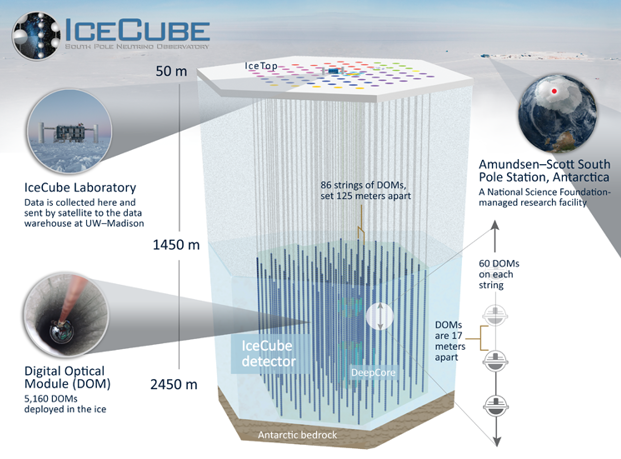
\includegraphics{images/icecube.png}
  \end{column}
  \end{columns}
\end{frame}

\begin{frame}\frametitle{IceTop}
  \begin{itemize}
    \item 81 Stationen oberhalb der Strings
    \item Dient als Veto und zur Kallibration
    \item Detektion von Teilchenschauern in der Atmosphere \"uber IceCube
    \item Sensitiv auf Energiebereich 300 TeV - 1 EeV
    \item Messung der Strahlkomposition
  \end{itemize}
\end{frame}

\begin{frame}\frametitle{DeepCore}
  \begin{itemize}
    \item kompaktes hexagonales Raster im inneren von IceCube
    \item senkt die Schwellenenergie auf ca. 10 GeV
    \item Studieren der Neutrinooszillation
  \end{itemize}
\end{frame}

\begin{frame}\frametitle{Wie funktioniert eine PMT?}
  \begin{columns}
    \begin{column}[c]{0.45\textwidth}
      \begin{itemize}
      \item PMT $\to$ Photomultiplier Tube
      \item $\gamma$ trifft auf Photokathode $\to$ Photoeffekt
      \item Prim\"arelektron l\"ost an jeder Dynode neue $e^{-}$ aus
      \item Abflie\ss en aller $e^{-}$ \"uber Widerstand $\to$ Spannungsabfall $\to$ Signal
      \item Verst\"arkung $\symup{\delta}$ $\approx$ $4^{10}$ \,-\, $6^{10}$
      \end{itemize}
    \end{column}
    \begin{column}[c]{0.45\textwidth}
      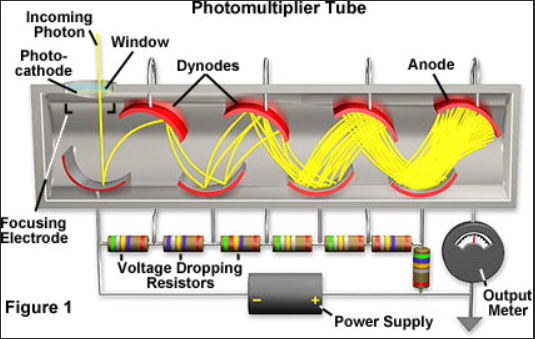
\includegraphics{images/pmt.png}
    \end{column}
  \end{columns}
\end{frame}

\begin{frame}\frametitle{Wie detektiert man Neutrinos eigentlich?}
  \begin{columns}
    \begin{column}[c]{0.45\textwidth}
      \begin{itemize}
      \item $\nu_{l}$ wechselwirkt mit Eis $\to$ geladenes Lepton
      \item Cherenkov Licht des geladenen Teilchens $\to$ Detektion durch PMTs
      \item speichern des timestamps von Signal des PMT
      \item Richtung und Geschwindigkeit des Neutrinos
      \end{itemize}
    \end{column}
    \begin{column}[c]{0.45\textwidth}
      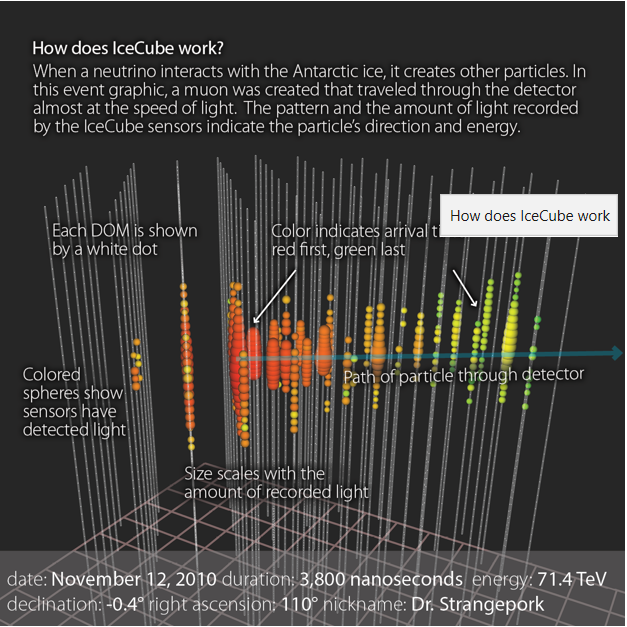
\includegraphics{images/signal_test.png}
    \end{column}
  \end{columns}
\end{frame}

\begin{frame}\frametitle{IceCube Upgrade}
  \begin{itemize}
    \item circa 140 zus\"atzliche strings mit 80 mDOMs
    \item detektorvolumen $\to$ 5-10 $\text{km}^{3}$
    \item mDOM: 24 PMTs mit nahezu 4$\pi$ Aufl\"osung
    \item gr\"o\ss eres Detektorvolumen $\to$ besser Energieaufl\"osung
  \end{itemize}
\end{frame}

\begin{frame}\frametitle{KM3NET}
  \begin{itemize}
    \item bla
  \end{itemize}
\end{frame}

\begin{frame}\frametitle{ANTARES}
% hier eventuell noch ein bild von antares rein
  \begin{block}{\"Uberblick}
    \begin{itemize}
      \item ANTARES $\hat{=}$ Astronomy with a Neutrino Telescope and Abyss environmental Research
      \item Inbetriebnahme 2008
      \item Unterwasser Cherenkovdetektor im Mittelmeer (40km vor der K\"uste Frankreichs bei Toulon)
      \item optimisiert f\"ur Myondetektion aus hochenergetischen Neutrinos
      \item Detektionsvolumen $approx$ gro\ss (richtigen wert nachschlagen!)
    \end{itemize}
  \end{block}
\end{frame}

\begin{frame}\frametitle{ANTARES}
\begin{block}{Detektor}
  \begin{columns}
    \begin{column}[c]{0.45\textwidth}
    \begin{itemize}
      \item circa 1000 PMTs
      \item 12 strings mit 350m l\"ange
      \item 25 storeys mit 3 OMs pro storey
    \end{itemize}
    \end{column}
    \begin{column}[c]{0.45\textwidth}
      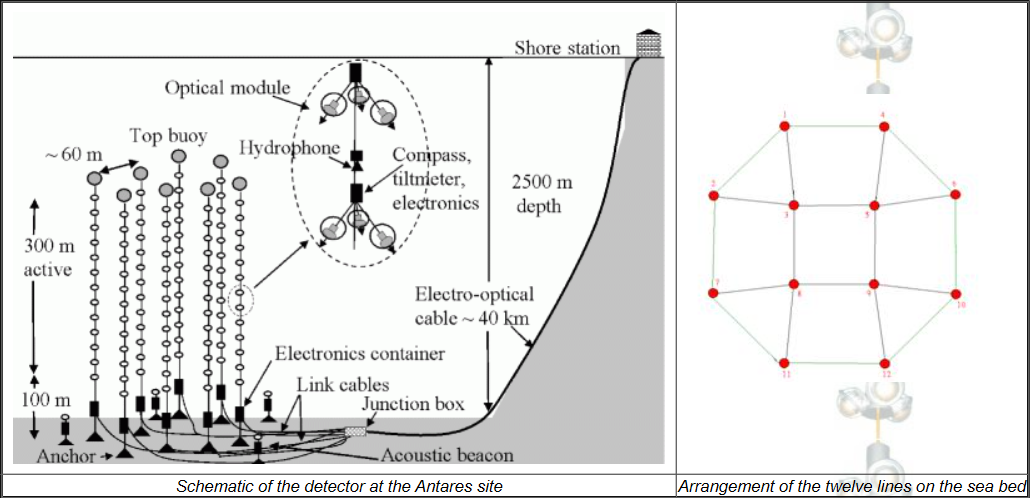
\includegraphics{images/antares1.png}
    \end{column}
  \end{columns}
\end{block}
\end{frame}

\begin{frame}\frametitle{ANTARES}
  \begin{block}{Detektion}
    \begin{itemize}
      \item geladene Str\"ome aus $\nu_{\mu}$ h\"aufig
      \item $\symup{E}(\mu^{-}) \approx \frac{1}{2}\times \symup{E}(\nu_{\mu})$
      \item geladene Str\"ome aus $\nu_{\text{e}}$ m\"oglich ab 100 GeV % energiedeosition besser als bei myon aber schlechte winkelaufloesung
      \item diskriminiere spuren von atmosph\"arischen neutrinos gegen neutrinos aus detektor
      \item $\to$ trajektorien "hoch" gegen "runter"
    \end{itemize}
  \end{block}
\end{frame}

\begin{frame}\frametitle{BAIKAL-GVD}
  \begin{block}{\"Uberblick}
    \begin{columns}
    \begin{column}[c]{0.45\textwidth}
      \begin{itemize}
        \item Giga-volume detector im Baikal See
        \item Projekt mit Beteiligung von 4 L\"andern
        \item 2016: Inbetriebnahme des ersten Clusters; 2021 8 Cluster aktiv
        \item Detektionsvolumen $approx$ $0.3 \text{km}^{3}$
        \item 8 Cluster; strings mit je 12 OMs pro Cluster + Mastermodule
        \item tiefe: 700m - 1240m u. NN.
        \item Pro: flacher Seeboden, klares Wasser, 1366m tief 
      \end{itemize}
    \end{column}
    \begin{column}[c]{0.45\textwidth}
      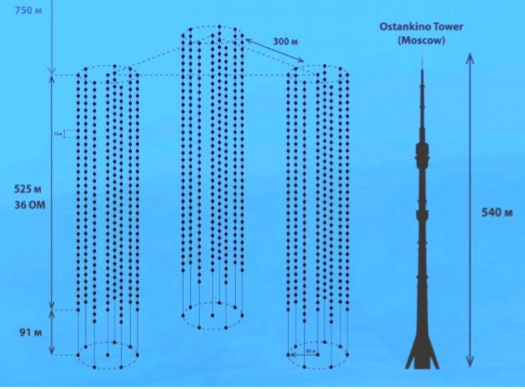
\includegraphics{images/baikal1.png}
    \end{column}
    \end{columns}
  \end{block}
\end{frame}

\begin{frame}\frametitle{BAIKAL-GVD}
  \begin{block}{Funktionsweise}
    \begin{columns}
    \begin{column}[c]{0.45\textwidth}
      \begin{itemize}
        \item Neutrino ww. $\to$ geladene Str\"ome
        \item Teilchen erzeugen Cherenkovlicht $\to$ OM-Informationen an Master; erzeugt timestamps
        \item Vereinigung der Clusterdaten zu vollst\"andiger Rekonstruktion der Teilchen
      \end{itemize}
    \end{column}
    \begin{column}[c]{0.45\textwidth}
      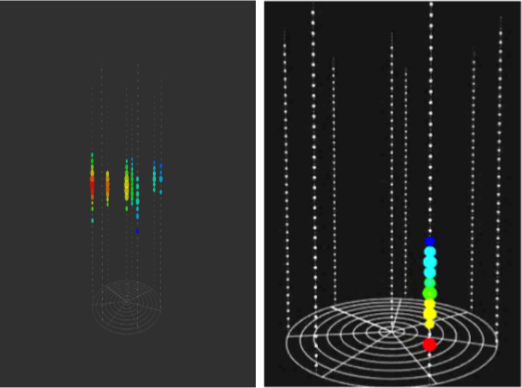
\includegraphics{images/baikal2.png}
    \end{column}
    \end{columns}
  \end{block}
\end{frame}


\begin{frame}\frametitle{STRAW}
  \begin{itemize}
    \item schona gelesenl; jetzt noch verstehen was die gemacht haben
  \end{itemize}
\end{frame}

\begin{frame}\frametitle{P-ONE}
  \begin{itemize}
    \item poster anschauen von jan
  \end{itemize}
\end{frame}

\begin{frame}\frametitle{Quellen}
\url{https://icecube.wisc.edu/science/icecube/detector} \\
\url{https://micro.magnet.fsu.edu/primer/digitalimaging/concepts/photomultipliers.html} \\
\url{http://antares.in2p3.fr/} \\
\url{https://ecap.nat.fau.de/index.php/research/neutrino-astronomy/antares-km3net/} \\
\url{http://www.km3net.org/} \\
\url{https://baikalgvd.jinr.ru/} \\
\url{https://masterok.livejournal.com/2364208.html} \\
\url{https://arxiv.org/pdf/1412.5106.pdf} \\
\url{https://www.epj-conferences.org/articles/epjconf/pdf/2019/14/epjconf_ricap2019_01015.pdf} \\
\url{https://pos.sissa.it/358/890/pdf} \\

\end{frame}

\end{document}